\section{Galaxy collision}
The parameters of the two galaxy models, the configuration of the methods used in the simulation, and the results are provided below in raw form.
\subsection{\texorpdfstring{\PThreeM{}}{P3M} method}
\begin{figure}[H]
    \centering
    \begin{subfigure}[b]{0.45\textwidth}
        \centering
        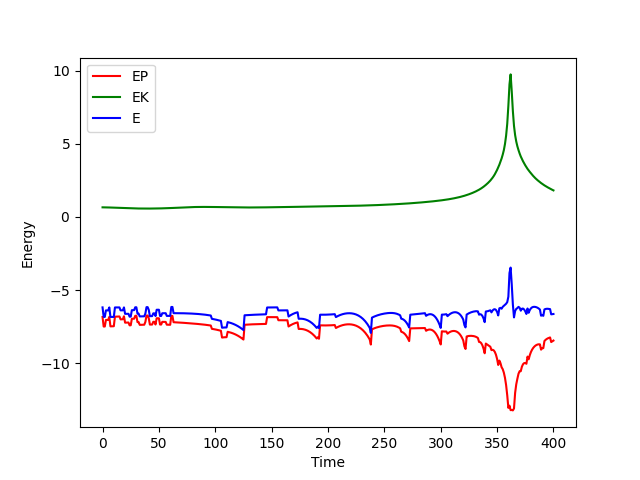
\includegraphics[width=\textwidth]{chapters/results/img/p3m-collision/energy.png}
        \caption{Energy}
        \label{fig:physical-quantities-p3m-collision-sub1}
    \end{subfigure}
    \hfill
    \begin{subfigure}[b]{0.45\textwidth}
        \centering
        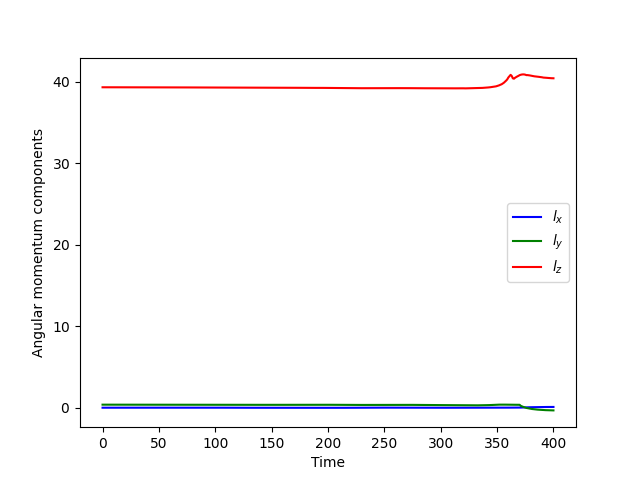
\includegraphics[width=\textwidth]{chapters/results/img/p3m-collision/angular-momentum.png}
        \caption{Angular momentum}
        \label{fig:physical-quantities-p3m-collision-sub2}
    \end{subfigure}

    \vspace{0.2cm}

    \begin{subfigure}[b]{0.45\textwidth}
        \centering
        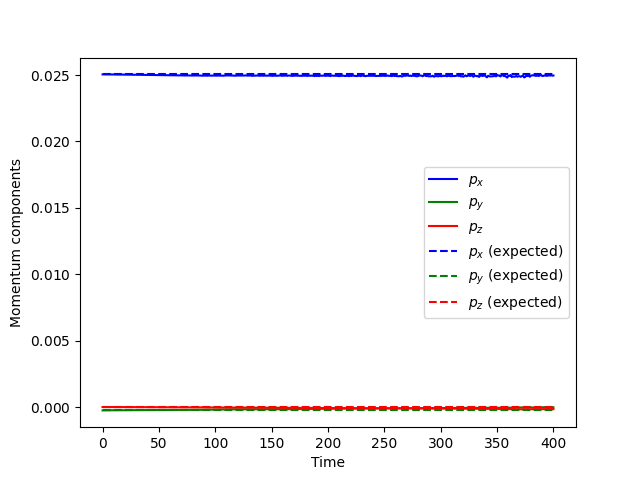
\includegraphics[width=\textwidth]{chapters/results/img/p3m-collision/momentum.png}
        \caption{Momentum; broken lines represent the expected momentum following \autoref{eq:expected-momentum-change}}
        \label{fig:physical-quantities-p3m-collision-sub3}
    \end{subfigure}

    \caption{Fundamental physical quantities describing the system over time in the \PThreeM{} method.
        Time is in Myr and the quantities are expressed in units consistent with \autoref{tab:galaxy-parameters-collision}}
    \label{fig:physical-quantities-p3m-collision}
\end{figure}

\begin{figure}[H]
    \centering
    \begin{subfigure}[b]{0.8\textwidth}
        \centering
        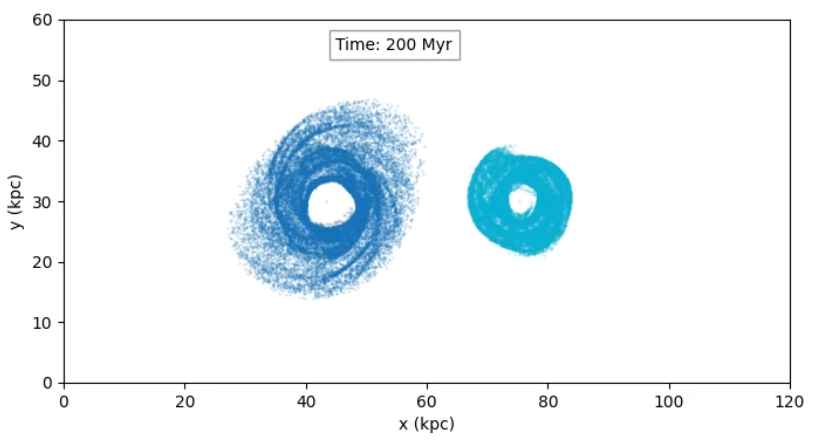
\includegraphics[width=\textwidth]{chapters/results/img/p3m-collision/200myr.png}
        \caption{$t=200\,\text{Myr}$}
        \label{fig:collision-p3m-sub1}
    \end{subfigure}

    \vspace{0.2cm}

    \begin{subfigure}[b]{0.8\textwidth}
        \centering
        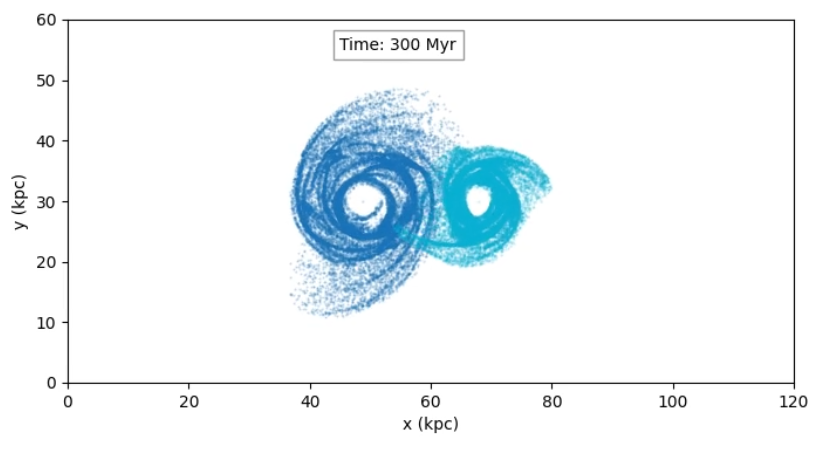
\includegraphics[width=\textwidth]{chapters/results/img/p3m-collision/300myr.png}
        \caption{$t=300\,\text{Myr}$}
        \label{fig:collision-p3m-sub2}
    \end{subfigure}

    \vspace{0.2cm}

    \begin{subfigure}[b]{0.8\textwidth}
        \centering
        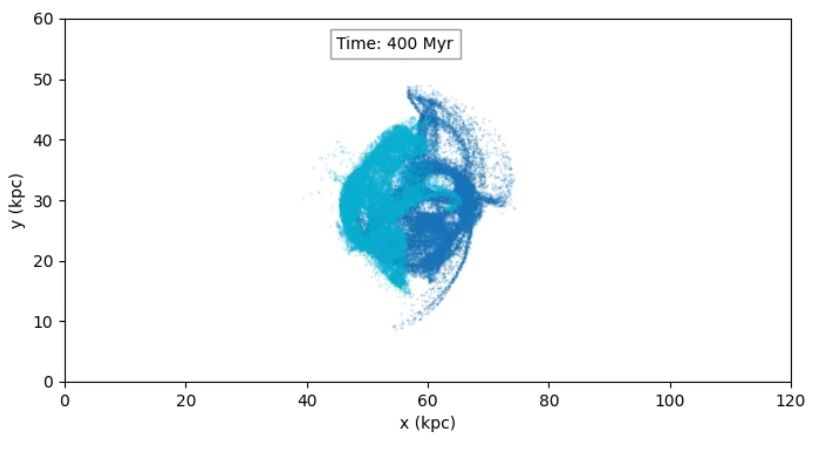
\includegraphics[width=\textwidth]{chapters/results/img/p3m-collision/400myr.png}
        \caption{$t=400\,\text{Myr}$}
        \label{fig:collision-p3m-sub3}
    \end{subfigure}

    \caption{Galaxy collision stage (\PThreeM{} method).}
    \label{fig:collision-p3m}
\end{figure}

\subsection{PM method}
\begin{figure}[H]
    \centering
    \begin{subfigure}[b]{0.5\textwidth}
        \centering
        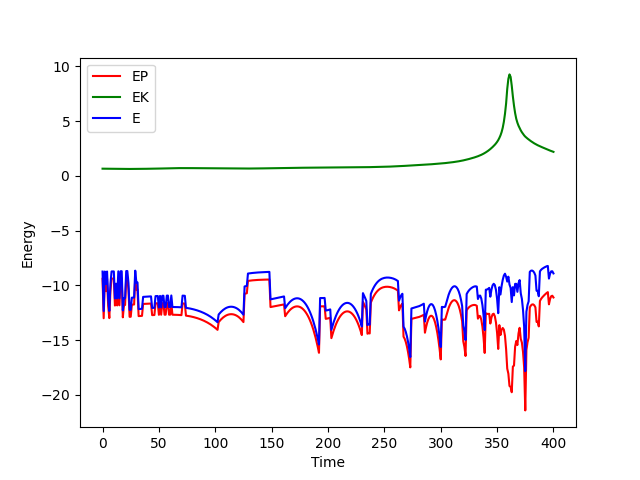
\includegraphics[width=\textwidth]{chapters/results/img/pm-collision/energy.png}
        \caption{Energy}
        \label{fig:physical-quantities-pm-collision-sub1}
    \end{subfigure}

    \vspace{0.2cm}

    \begin{subfigure}[b]{0.5\textwidth}
        \centering
        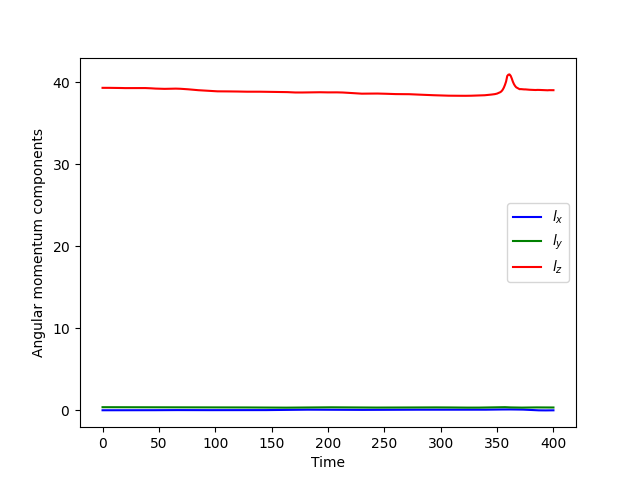
\includegraphics[width=\textwidth]{chapters/results/img/pm-collision/angular-momentum.png}
        \caption{Angular momentum}
        \label{fig:physical-quantities-pm-collision-sub2}
    \end{subfigure}

    \vspace{0.2cm}

    \begin{subfigure}[b]{0.5\textwidth}
        \centering
        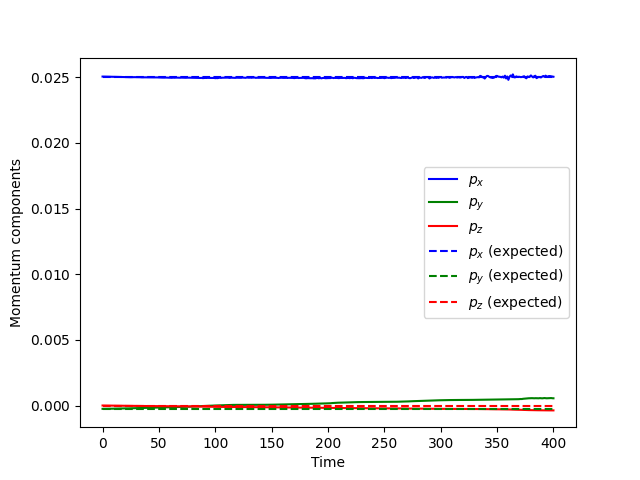
\includegraphics[width=\textwidth]{chapters/results/img/pm-collision/momentum.png}
        \caption{Momentum; broken lines represent the expected momentum following \autoref{eq:expected-momentum-change}}
        \label{fig:physical-quantities-pm-collision-sub3}
    \end{subfigure}

    \caption{Fundamental physical quantities describing the system over time in the PM method.
        Time is in Myr and the quantities are expressed in units consistent with \autoref{tab:galaxy-parameters-collision}}
    \label{fig:physical-quantities-pm-collision}
\end{figure}

\begin{figure}[H]
    \centering
    \begin{subfigure}[b]{0.8\textwidth}
        \centering
        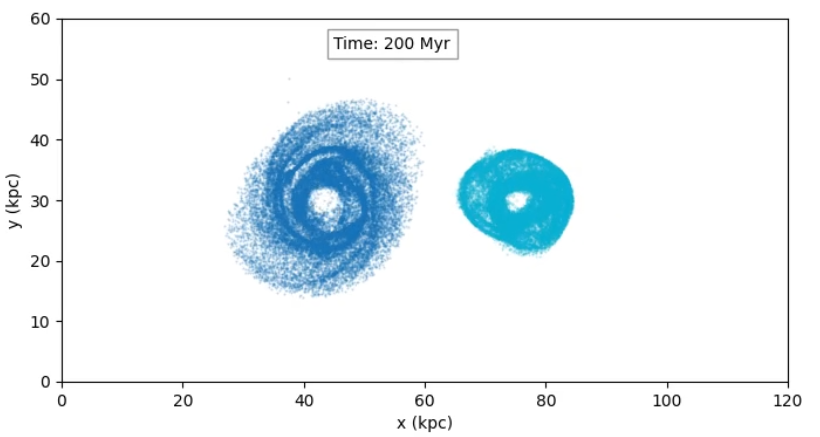
\includegraphics[width=\textwidth]{chapters/results/img/pm-collision/200myr.png}
        \caption{$t=200\,\text{Myr}$}
        \label{fig:collision-pm-sub1}
    \end{subfigure}

    \vspace{0.2cm}

    \begin{subfigure}[b]{0.8\textwidth}
        \centering
        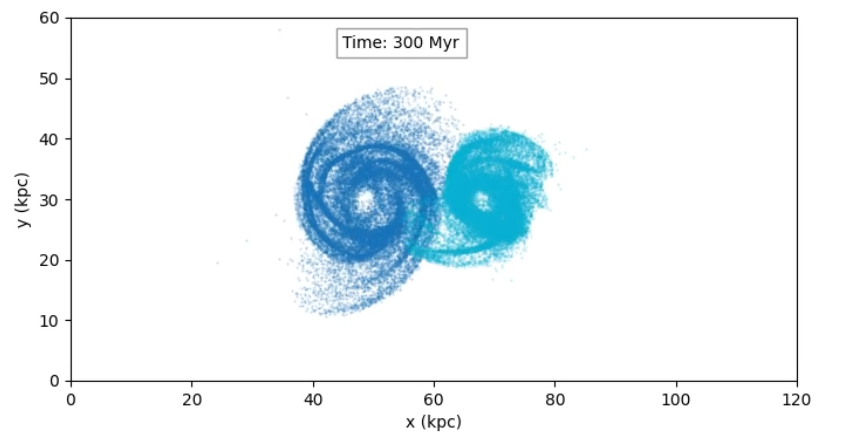
\includegraphics[width=\textwidth]{chapters/results/img/pm-collision/300myr.png}
        \caption{$t=300\,\text{Myr}$}
        \label{fig:collision-pm-sub2}
    \end{subfigure}

    \vspace{0.2cm}

    \begin{subfigure}[b]{0.8\textwidth}
        \centering
        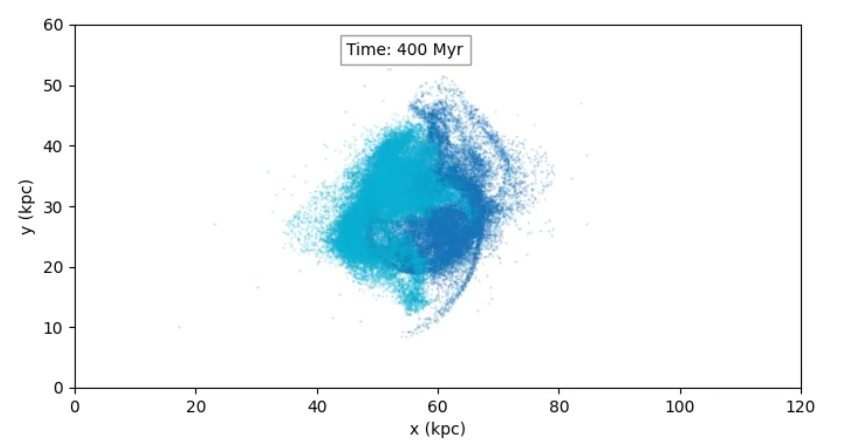
\includegraphics[width=\textwidth]{chapters/results/img/pm-collision/400myr.png}
        \caption{$t=400\,\text{Myr}$}
        \label{fig:collision-pm-sub3}
    \end{subfigure}

    \caption{Galaxy collision stage (PM method).}
    \label{fig:collision-pm}
\end{figure}